% \iffalse
\let\negmedspace\undefined
\let\negthickspace\undefined
\documentclass[journal,12pt,twocolumn]{IEEEtran}
\usepackage{amssymb}
\usepackage{cite}
\usepackage{amsmath,amssymb,amsfonts,amsthm}
\usepackage{algorithmic}
\usepackage{graphicx}
\usepackage{textcomp}
\usepackage{xcolor}
\usepackage{txfonts}
\usepackage{listings}
\usepackage{enumitem}
\usepackage{mathtools}
\usepackage{gensymb}
\usepackage{comment}
\usepackage[breaklinks=true]{hyperref}
\usepackage{tkz-euclide} 
\usepackage{listings}
\usepackage{gvv}                                        
\def\inputGnumericTable{}                                 
\usepackage[latin1]{inputenc}                                
\usepackage{color}                                            
\usepackage{array}                                            
\usepackage{longtable}                                       
\usepackage{calc}                                             
\usepackage{multirow}                                         
\usepackage{hhline}                                           
\usepackage{ifthen}                                           
\usepackage{lscape}
\usepackage{pgfplots}
\newtheorem{theorem}{Theorem}[section]
\newtheorem{problem}{Problem}
\newtheorem{proposition}{Proposition}[section]
\newtheorem{lemma}{Lemma}[section]
\newtheorem{corollary}[theorem]{Corollary}
\newtheorem{example}{Example}[section]
\newtheorem{definition}[problem]{Definition}
\newcommand{\BEQA}{\begin{eqnarray}}
\newcommand{\EEQA}{\end{eqnarray}}
\newcommand{\define}{\stackrel{\triangle}{=}}
\theoremstyle{remark}
\newtheorem{rem}{Remark}
\begin{document}

\bibliographystyle{IEEEtran}
\vspace{3cm}

\title{NCERT Discrete-10.5.3-7}
\author{EE22BTECH11004 - Allu Lohith}

\maketitle
\newpage
\bigskip

\renewcommand{\thefigure}{\theenumi}
\renewcommand{\thetable}{\theenumi}
\begin{enumerate}
\item
Find the sum of the first 22 terms of an AP in which $d = 7$ and the 22nd term is 149.
\solution

\begin{table}[h!]
\centering
\begin{table}[ht]
    \centering
    \begin{tabular}{|c|c|c|}
        \hline
        Parameter & Value & Description \\
        \hline
        $x(0)$ & 5 & First term of AP \\
        $d$ & 1.75 & Common difference of AP \\
        $x(n)$ & 20.75 & $n^{th}$ term of AP \\
        \hline
    \end{tabular}
    \vspace{2mm}
    \caption{Parameter List}
    \label{tab:simple.10.5.2.20}
\end{table}

\vspace{0.5cm}
\caption{\normalsize Parameters}
\end{table}

Now, the $22^{nd}$ term means $x(21)$, so

\begin{align}
x(21) &= \brak{x(0)+nd}u\brak {21}\\
149 &= \brak{x(0)+21\brak 7}\brak 1\\
x(0) &= 2    
\end{align}
The standard $z$ transforms,
\begin{align}
    u \brak n &\stackrel{z}{\longleftrightarrow} \frac{1}{1-z^{-1}}, \abs z >1\\
   n u\brak n &\stackrel{z}{\longleftrightarrow} \frac{z^{-1}}{\brak{1-z^{-1}}^2}, \abs z >1
\end{align}
The general term is $x(n)=\brak {2+7n}u\brak n$,
The $z$ transform of the general term is 
\begin{align}
X(z)&= \frac{x(0)}{1-z^{-1}}+\frac{dz^{-1}}{\brak{1-z^{-1}}^2} \\
&=\frac{2}{1-z^{-1}}+\frac{7z^{-1}}{{\brak{1-z^{-1}}^2}}\\
&=\frac{2+5z^{-1}}{\brak{1-z^{-1}}^2} ; \quad \abs z>1
\end{align}
On convolution for finding the sum
\begin{align}
    y(n)=x(n)\ast u(n)
\end{align}
On z-transform, 
\begin{align}
Y(z)&=X(z)\cdot U(z)\\
    &=\brak{\frac{{2+5z^{-1}}}{{(1-z^{-1})^2}}} \cdot \frac{1}{{1-z^{-1}}}\\
  \implies Y(z)  &= \frac{2+5z^{-1}}{\brak{1-z^{-1}}^3} ; \quad \quad \abs z>1
\end{align}
Using Contour integration to find the inverse z-transform,
\begin{align}
    y(n)&=\oint_c Y(z)\cdot z^{n-1}dz\\
    y(21)&=\oint_c \frac{2+5z^{-1}}{\brak{1-z^{-1}}^3}\cdot z^{20}dz
\end{align}
We can observe there are three poles and thus m = 3,
\begin{align}
    y\brak{21}&=\frac{1}{\brak{m-1}!} \lim_{z \to a} \frac{d^{m-1}}{dz^{m-1}}\brak{\brak{z-a}^mf\brak z}\\
    &=\frac{1}{2!}\lim_{z \to 1} \frac{d^2}{dz^2} \brak{\brak{z-1}^3\cdot \frac{2+5z^{-1}}{\brak{1-z^{-1}}^3}\cdot \brak{z^{20}}}\\
    &=\frac{1}{2}\brak{1012+2310}\\
    \implies y \brak{21}&=1661
\end{align}
\begin{figure}[h]
    \centering  

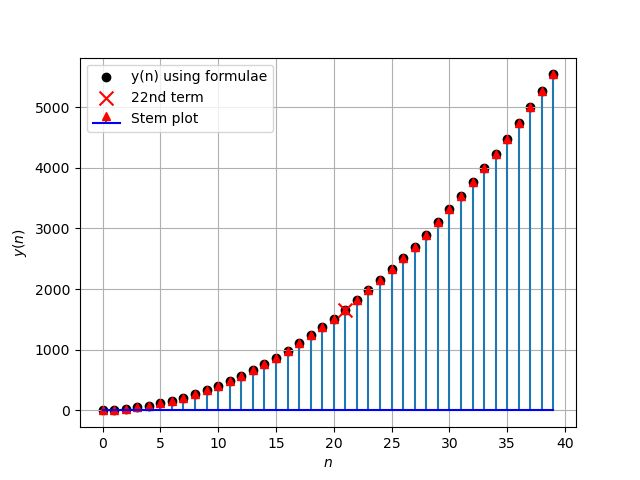
\includegraphics[width=\columnwidth]{fig/plot.png}

\begin{center}
    \caption{Simulation v/s theoretical}
\end{center}
    
    \label{fig:}
\end{figure}


\end{enumerate}
\end{document}
